\section{Comparing Models on Full Statistics Signal}
So far in the analysis I have only tested on a subset of the signal, which I have called the original signal set. In this section 
I will extend my search to include the full signal set displayed in figure \ref{fig:nrSignal}. The full signal set consists of 89 mass 
combinations compared to the original 30, and extends the mass ranges to $\tilde{\chi}_1 \in [0-400]GeV$ and $\tilde{\chi}_2 \in [200-800]GeV$.
In the figures to come, I have included a turquoise band around all combinations with a significance of over 1.64 (see section \ref{subsec:Sensitivity}).
When comparing the results, we are not only interested in how sensitive the models are for each combination individually, but also with how many combinations 
they were able to achieve a sensitivity of over 1.64. However, similarly to previous results, the significance does not include any uncertainty.
\\
I will not apply all previously tested models to the full statistics signal set. Instead, I will only apply the models I found most ideal for this analysis, based 
on the tests performed in the previous sections. I decided to choose one model from each "type"\footnote{By network type, I am referring to either the ordinary dense network, the 
\ac{PNN} or an ensemble. } of network. Based on the results in section \ref{sec:Ensemble}, where I compared the different ensemble methods, I found the maxout model to be 
the top performer. Likewise, in section \ref{sec:PCA} I found that both maxout and the \ac{PNN}, preferred to utilize data with a \ac{PCA}. Therefore, I will utilize the maxout model 
and \ac{PNN} model defined in section \ref{subsec:arch}, with the use of \ac{PCA}. Finally, I will include the ordinary dense \ac{NN} for the sake of diversity.
\\
In figure \ref{fig:NN_FS_MLMGridSig}, I have drawn a grid displaying the sensitivity of an ordinary dense \ac{NN}, on the full statistics signal set. Again, we observe that higher statistics
mass combinations, result in a higher significance. Additionally, the dense \ac{NN} was able to achieve a sufficient significance for over 38 mass combinations, all between the ranges of 
$\tilde{\chi}_1 \in [0-250]GeV$ and $\tilde{\chi}_2 \in [200-600]GeV$. What is even more interesting, is that by comparing the results on the full set with the results on the original 
set (see figure \ref{fig:NNGridSig}), we notice that the network was able to improve its sensitivity on every single mass combination from the original signal set. This is yet another 
indication that the deep networks are able to exploit overlapping regions in the feature space between nearby combinations.
\begin{figure}
    \makebox[\linewidth][c]{%
    \centering
    \begin{subfigure}{.85\textwidth}
        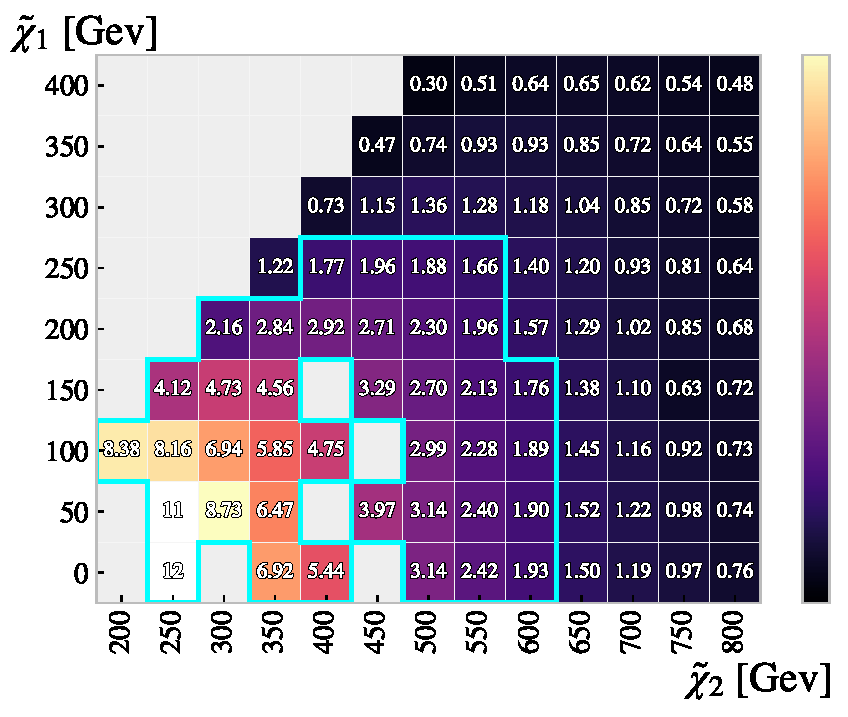
\includegraphics[width=\textwidth]{Figures/MLResults/NN/SUSY/Grid/FS/NN_FS_MLMGridSig.pdf}
    \end{subfigure}
    }
    \caption{A grid displaying the achieved significance on the full statistics signal set, using the signal region 
    created by the \ac{NN} network.}
    \label{fig:NN_FS_MLMGridSig}
\end{figure}

\begin{figure}
    \makebox[\linewidth][c]{%
    \centering
    \begin{subfigure}{.85\textwidth}
        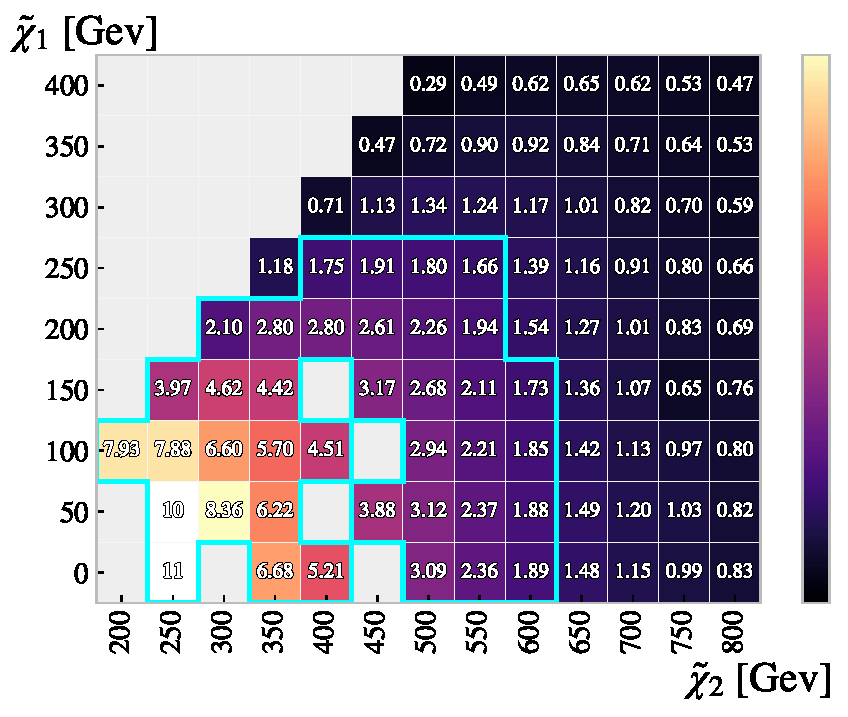
\includegraphics[width=\textwidth]{Figures/MLResults/NN/SUSY/Grid/FS/MaxOutPCA_FS_MLMGridSig.pdf}
    \end{subfigure}
    }
    \caption{A grid displaying the achieved significance on the full statistics signal set, using the signal region 
    created by the \emph{MaxOut} network.}
    \label{fig:MaxOutPCA_FS_MLMGridSig}
\end{figure}

\begin{figure}
    \makebox[\linewidth][c]{%
    \centering
    \begin{subfigure}{.85\textwidth}
        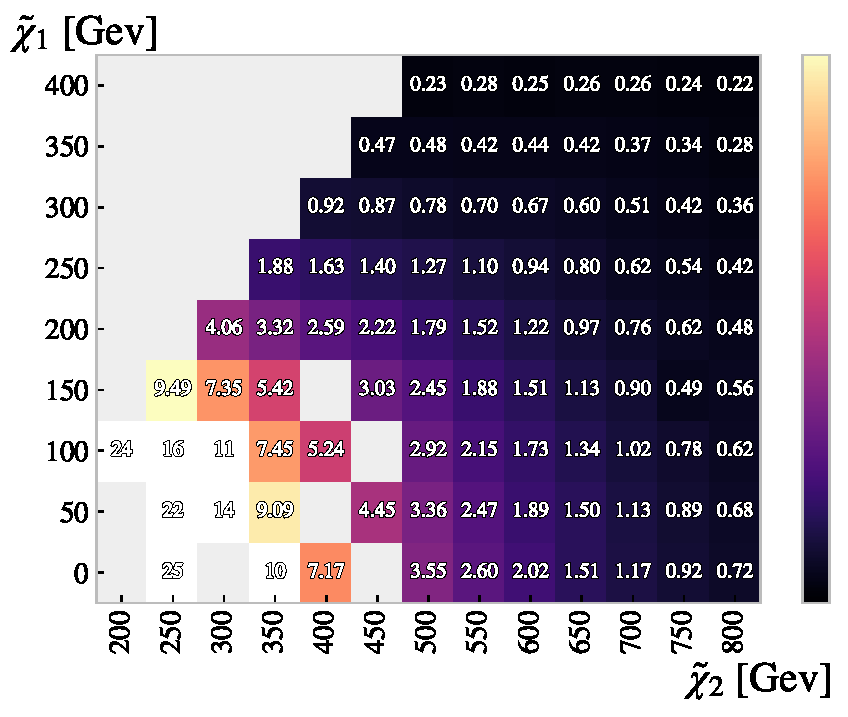
\includegraphics[width=\textwidth]{Figures/MLResults/NN/SUSY/Grid/FS/PNNPCA_FS_MLMGridSig.pdf}
    \end{subfigure}
    }
    \caption{A grid displaying the achieved significance on the full statistics signal set, using the signal region 
    created by the \emph{PNN} network.}
    \label{fig:PNNPCA_FS_MLMGridSig}
\end{figure}